\section{Grafos dirigidos}
\stepcounter{sec}

Hasta ahora hemos utilizado los grafos para modelar relaciones simétricas, pero en general este no tiene por qué ser el caso. Por ejemplo, en algunas redes se puede \textit{seguir} a alguien y éste no necesariamente te sigue. En estos casos decimos que la relación va en una \textit{dirección}. Esto se refleja gráficamente partiendo de la idea de un grafo: Solo hace galta agregar la dirección en los lados, lo que indica el orden de la relación.

\begin{defn}
    Un \ul{digrafo} o \ul{grafo dirigido}, es una tripleta $G = ( V(G), E(G), f_G)$ en el cual $V(G)$ y $E(G)$ son conjuntos (de vértices y lados) y $f_G: E(G) \rightarrow V(G) \times V(G)$.
    
    Si $(v,w) = f_G(e)$ para algún $e \in E(G)$, entonces decimos que $v$ es la \ul{cola} de $e$, y $w$ es la \ul{cabeza} de $e$. En este caso, escribimos $v \rightarrow w$ y también decimos que $v$ es \ul{predecesor} de $w$, y $w$ es \ul{sucesor} de $v$.
    
    Los lados cuyas imágenes tienen la forma $(v,v)$ son \ul{bucles} y si $f_G$ no es inyectiva, decimos que $G$ tiene lados \ul{múltiples}. Si $f_G$ es inyectiva, entonces decimos que $G$ es simple. Se observa que un digrafo simple $G$ puede tener bucles. Como antes, denotaremos $|V(G)| = n(G)$, $|E(G)| = e(G)$.
\end{defn}

\begin{ejem}
    \begin{marginfigure}
        % Falta hacer el digrafo
        \centering
        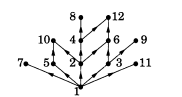
\includegraphics{img/digrafo.PNG}
        \caption{Ejemplo de digrafo.}
        \label{fig:digrafo}
    \end{marginfigure}
    
    Vemos en la figura \ref{fig:digrafo}~que $V(G) = [12]$, $E(G)$ está formado por las flechas y $f_G(e) = (t,h)$ si $h/t$ es primo. En este caso, el digrafo es simple.
\end{ejem}

\begin{ejem}
    \begin{marginfigure}
        % Falta hacer el digrafo
        \centering
        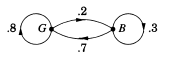
\includegraphics{img/markov.PNG}
        \caption{Cadena de Markov.}
        \label{fig:markov}
    \end{marginfigure}
    
    Los digrafos son útiles para modelar sistemas en los que los vértices representan estados, y los lados representan transición entre ellos. Un sistema cuyos estados cambian de forma aleatoria se llama \textbf{cadena de Markov}. Por ejemplo, en la figura \ref{fig:markov}~tenemos representados a los estados del tiempo con $G$ (bueno) y $B$ (malo). Las probabilidades son:
    
    \begin{enumerate}
        \item Que un día bueno siga siendo bueno: $0.8$.
        \item Que un día bueno se haga malo: $0.2$.
        \item Que un día malo siga siendo malo: $0.3$.
        \item Que un día malo se haga bueno: $0.7$.
    \end{enumerate}
\end{ejem}

\begin{defn}
    Dado un digrafo $D$, el \ul{grafo base} $G$ de $D$ se obtiene con los vértices de $D$ y considerando los lados sin tomar en cuenta el orden de los pares.
\end{defn}

\begin{defn}
    Un digrafo simple es un \ul{camino} si sus vértices se pueden ordenar de la forma $v_1, v_2, \dots, v_n$ con $v_i \rightarrow v_j$ si y sólo si $j = i+1$. En este caso decimos que se trata de un camino de $v_1$ a $v_n$.
    
    Un digrafo simple es un \ul{ciclo} si sus vértices se pueden ordenar de la forma $v_1, \dots, v_n$ con $v_i \rightarrow v_j$ si y sólo si $j = i+1$ ó $i=n$ y $j=1$.
    
    Otros conceptos visto para grafos son análogos para grafos:
    
    \begin{itemize}
        \item Subdigrafo.
        \item Isomorfismo (digrafos isomorfos, clases de isomorfismo).
        \item Descomposición de digrafos.
        \item Unión de digrafos.
    \end{itemize}
\end{defn}

Otros conceptos requieren modificaciones, o tienen algunas diferencias:

\begin{defn}
    Dado un digrafo $G$:
    
    \begin{itemize}
        \item Una \ul{matriz de incidencia} (si $G$ no tiene bucles) $M(G)$ está dada por $m_{ij} = 1$ si $x_i$ es la cola de $e_j$ y $m_{ij} = -1$ si $v_i$ es la cabeza de $e_j$.
        \item Una \ul{matriz de adyacencia} $A(G)$ está dada por $a_{ij} =$~cantidad de lados correspondientes a $v_i \rightarrow v_j$.
    \end{itemize}
    
    \begin{figure}
        \centering
        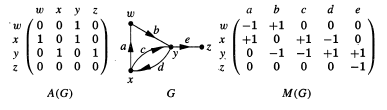
\includegraphics{img/matrices.PNG}
        \caption{}
        \label{fig:matrices}
    \end{figure}
\end{defn}

\begin{defn}
    Dados dos vértices $v,w$ de un digrafo, es posible que existe un camino de $v$ a $w$ y que no exista un camino de $w$ a $v$. Dado un digrafo $G$ con grafo base $G$, decimos que
    
    \begin{enumerate}
        \item $D$ es \ul{débilmente conexo} si $G$ es conexo.
        \item $D$ es \ul{conexo (o fuertemente conexo)} si para cada par ordenado de vértices $v,w$, existe un camino de $v$ a $w$ en $D$.
    \end{enumerate}
\end{defn}

\subsection{Grados y suceciones gráficas}
\stepcounter{subsec}

\begin{defn}
    Dados un digrafo $G$ y $v \in V(G)$,
    
    \begin{itemize}
        \item El \ul{grado de entrada} de $v$ en $G$ es la cantidad $d_G^-(v)$ de lados que tienen a $v$ como cabeza.
        \item El \ul{grado de salida} de $v$ en $G$ es la cantidad $d_G^+(v)$ de lados que tienen a $v$ como cola.
        \item El conjunto de \ul{predecesores} de $v$ es $N_G^-(v) \{w \in V(G) : w \rightarrow v\}$.
        \item El conjunto de \ul{sucesores} de $v$ es $N_G^+(v) \{w \in V(G) : v \rightarrow w\}$.
        \item $\delta^-(G) = \min \{d_G^-(w) : w \in V(G)\}$.
        \item $\Delta^-(G) = \max \{d_G^-(w) : w \in V(G)\}$.
        \item $\delta^+(G) = \min \{d_G^+(w) : w \in V(G)\}$.
        \item $\Delta^-(G) = \max \{d_G^+(w) : w \in V(G)\}$.
    \end{itemize}
\end{defn}

\begin{teo}
    En un digrafo $G$, tenemos que
    
    \[
    \sum_{v \in V(G)} d^+(v) = e(G) = \sum_{v \in V(G)} d^-(v)
    \]
\end{teo}

\begin{proof}
    Cada lado tiene exactamente una sola cola y una sola cabeza.
\end{proof}

Ahora, si quisiéramos definir sucesiciones (di)gráficas, tendrían que ser sucesiones de pares de números $(d_1^+,d_1^-), \dots, (d_n^+,d_n^-)$.

\begin{teo}
    Una lista de pares ordenados de enteros no negativos es realizable por un digrafo sii la suma de las primeras coordenadas es igual a la suma de las segundas coordenadas.
\end{teo}

\begin{proof}
    La condición es necesaria porque todo lado tiene una cola y una cabeza, contribuyendo cada uno exactamente uno a cada suma.
    
    Para ver la suficiencia, consideremos las parejas
    
    \[
    \{ (d_i^+, d_i^-) : 1 \leq i \leq n \}
    \]
    
    \noindent y los vértices $v_1, \dots, v_n$. Sea ahora $\sum_{j=1}^n d_j^- = \sum_{i=1}^n d_i^+ = m$. Consideremos los $n$ vértices y construyamos $m$ pares ordenados de la siguiente manera:
    
    Para cada $i$, se coloca $i$ en las primeras $d_i^+$ coordenadas. Para cada $j$, se coloca $-j$ en las primeras $d_j^-$ coordenadas. Para cada $(i,-j)$ agregamos un lado de $v_i$ a $v_j$. El digrafo resultante realiza $(d_1^+, d_1^-), \dots, (d_n^+, d_n^-)$.
    
    Así, queda demostrado el teorema.
\end{proof}

Para este teorema permitimos lados múltiples, ¿cómo podemos estudiar una versión análoga para digrafos simples?. Nos valdremos de una técnica que hace uso de los grafos bipartitos:

\begin{defn}
    El \ul{split} de un digrafo $D$ es un grafo bipartito $G$ cuyos conjuntos bipartitos $V^+$, $V^-$ son copias de $V(D)$. Para cada vértice $x \in V(D)$, tenemos un vértice $x^+ \in V^+$ y un vértice $V^- \in V^-$. Para cada lado $u,v \in E(D)$, hay un lados con extremos $u^+, v^- \in G$.
\end{defn}

\begin{figure}
    \centering
    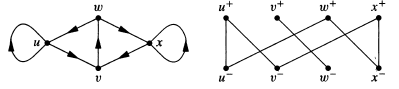
\includegraphics{img/split.PNG}
    \caption{Ejemplo de split.}
    \label{fig:split}
\end{figure}

En la figura \ref{fig:split}~se observa que los grados en $G$ corresponden a los grados de salida y entrada en $D$.

Más aún, dado un grafo bipartito $G$ con bipartición $X$, $Y$ tal que $|X| = |Y| = n$, se puede revertir el proceso para obtener un digrafo $D$ tal que $G$ sea su split. Aquí se ve claro por qué permitimos bucles en los digrafos simples.

Entonces, dada $(d_1^+,d_1^-), \dots, (d_n^+,d_n^-)$ tal que la suma de las primeras coordenadas es igual a la suma de las segundas, existe un digrafo simple que la realiza si y sólo si existe un grafo $G$, bipartito con particiones $X$ e $Y$ tal que $|X| = |Y| = n$, donde los $d_j^+$ son grados en $X$ y los $d_j^-$ son los grados en $Y$.

\subsection{El digrafo de De Bruijin}
\stepcounter{subsec}

Es sencillo dar los conceptos de \textit{paseo} y \textit{recorrido} para digrafos. A partir de allí se puede definir de inmediato \textit{recorridos eulerianos}, \textit{circuitos eulerianos} y \textit{digrafos eulerianos}. De hecho, para obtener una caracterización de los digrafos eulerianos en función de los grados de los vértices, basta con un par de resultados sencillos.

\begin{lem}
    Si $G$ es un digrafo tal que $\delta^+(G) \geq 1$ ó $\delta^-(G) \geq 1$, entonces $G$ tiene un ciclo.
\end{lem}

\begin{proof}
    Supongamos que $G$ es un digrafo para el cual $\delta^+(G) \geq 1$. Sea $P$ un camino maximal en $G$. Si $u$ es el último vértice de $P$, $u$ tiene un sucesor en $P$. De esta manera, obtenemos un ciclo en $G$. Para demostrar cuando $\delta^-(G) \geq 1$, el razonamiento es totalmente análogo.
\end{proof}

\begin{teo}
    Un digrafo $G$ es euleriano sii para cada $v \in V(G)$ vale $d^+(G) = d^-(G)$ y el grado base de $G$ a lo sumo tiene una componente no trivial.
\end{teo}

\begin{proof}
    Queda como ejercicio. Se demuestra usando inducción y el lema anterior.
\end{proof}

Ahora, pasemos a observar la siguiente sucesión binaria:

\[
0000111101100101
\]

Esta cumple con lo siguiente:

\begin{enumerate}
    \item Cada bloque de $4$ dígitos consecutivos es distinto.
    \item Si esto se ve de forma cíclica, es aparente que están todos los $4$-bloques posibles.
\end{enumerate}

Esto es un ejemplo de lo que se conoce como \textbf{ciclo de De Bruijin}. En general, un ciclo de De Bruijin es una cadena de longitud $2^n$ tal que, vista de forma cíclica, contiene todos los $n$-bloques binarios distintos. Dado $n$, ¿existe un ciclo de De Bruijin para ese $n$? Si es así, ¿cómo se puede construir?

Volvamos al ejemplo que dimos anteriormente ($n=4$). Usaremos un digrafo $D_4$ construído de la siguiente manera:

\begin{enumerate}
    \item Los vértices de $D_4$ son cadenas binarias de $3$ dígitos.
    \item $u \rightarrow v$ si los últimos $2$ dígitos de $u$ coinciden con los primeros de $v$.
    \item Etiquetamos el lado $u \rightarrow v$ con el último dígito de $v$.
    \item $D_4$ es euleriano.
    \item Las etiquetas de los lados de cualquier circuito euleriano en $D_4$ forman un ciclo de De Bruijin.
\end{enumerate}

\begin{figure}
    \centering
    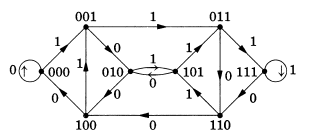
\includegraphics{img/de-bruijin.PNG}
    \caption{Ciclo de De Bruijin $D_4$.}
    \label{fig:de-bruijin}
\end{figure}

Vemos que en general, dado $n$ tenemos que los vértices de $D_n$ son las cadenas binarias con $n-1$ dígitos, si $u \rightarrow v$ los últimos $n-2$ dígitos coinciden con los primeros $n-2$ de $v$, y se etiqueta al lado $u \rightarrow v$ con el último dígito de $v$.

Esto nos motiva a el siguiente teorema:

\begin{teo}
    Para cada $n$, $D_n$ es euleriano y las etiquetas de cada ciclo euleriano en $D_n$ definen un diclo de De Bruijin.
\end{teo}

\begin{proof}
    Sea $D_n$. Entonces al agregar $0$ o $1$ al final de un vértice y eliminar el primero, obtenemos un sucesor, por lo que $d^+(v) = 2$ para todo $v \in V(D_n)$, y cada vértice es sucesor de otro que comienza en $1$ y otro que comienza en $0$, por lo tanto $d^-(v) = 2$. Entonces $d^+(v) = d^-(v) = 2$ para cada $v$. Más aún, dado un vértice $b_1b_2 \dots b_{n-1}$ podemos llegar a él desde cualquier otro vértice, siguiente los lados etiquetados con $b_1, b_2, \dots$. Por lo tanto $D_n$ es euleriano.
    
    Ahora, para llegar a un vértice $v = b_1b_2 \dots b_{n-1}$, debe haber sido a través de lados con etiquetas $b_1, \dots, b_{n-1}$. Si desde $v$ se usa un lado etiquetado con $b_n$, se obtiene la cadena $b_1b_2 \dots b_n$. Como los vértices son cadenas distintas, tenemos todas las cadenas binarias (distintas) de longitud $n$ usando un ciclo euleriano.
\end{proof}

\subsection{Orientaciones y torneos}
\stepcounter{subsec}

Para introducir el concepto de torneos, presentamos el siguiente problema:

\begin{prob}
    En varios deposrtes se hacen torneos tipo \textit{round robin}: cada equipo se enfrenta a otro sólo una vez y no hay empates. Si son $n$ equipos, ¿cuántos resultados son posibles en un torneo así?
    
    Podemos modelar el resultado con un digrafo:
    
    \begin{itemize}
        \item Cada equipo es un vértice.
        \item Todos los vértices son vecinos dos a dos.
        \item Si $x$ derrota a $y$ entonces escribimos $x \rightarrow y$.
        \item En cada juego hay dos posibilidades $x \rightarrow y$ ó $y \rightarrow x$.
    \end{itemize}
    
    \begin{marginfigure}
        \centering
        \begin{tikzpicture}
            \GraphInit[vstyle=Classic]
            \SetVertexNoLabel
            \grComplete[RA=2]{6}
            \tikzset{EdgeStyle/.append style = {red}}
            \Edge[style={->}, color=red](a0)(a1)
            \Edge[style={->}, color=red](a0)(a2)
            \Edge[style={->}, color=red](a0)(a4)
            \Edge[style={->}, color=red](a5)(a0)
            \Edge[style={->}, color=red](a3)(a0)
            \Edge[style={->}, color=red](a2)(a1)
            \Edge[style={->}, color=red](a1)(a3)
            \Edge[style={->}, color=red](a1)(a4)
            \Edge[style={->}, color=red](a5)(a1)
            \Edge[style={->}, color=red](a3)(a2)
            \Edge[style={->}, color=red](a2)(a4)
            \Edge[style={->}, color=red](a5)(a2)
            \Edge[style={->}, color=red](a4)(a5)
            \Edge[style={->}, color=red](a5)(a3)
            \Edge[style={->}, color=red](a3)(a4)
        \end{tikzpicture}
        \caption{Torneo de 6 vértices.}
        \label{fig:torneo}
    \end{marginfigure}
    
    Observémos las características del digrafo \ref{fig:torneo}~, no hay lados múltiples, no hay bucles y cada vértice es vecino de todos los demás.
\end{prob}

Todo esto nos permite establecer las siguientes definiciones:

\begin{defn}
    Una \ul{orientación} de un grafo $G$ es un digrafo $D$ obtenido a partir de $G$ al escoger una orientación $x \rightarrow y$ ó $y \rightarrow x$ para cada lado $xy \in E(G)$. Un \ul{grafo orientado} es una orientación de un grafo simple sin bucles. Un \ul{torneo} es una orientación de un grafo completo.
\end{defn}

\begin{prob}
    ¿En general, cuántos digrafos con $n$ vértices hay?: En primer lugar, hay $n^2$ pares ordenados de vértices (permitiendo bucles). Un digrafo simple permite bucles pero usa cada par ordenado a lo sumo una vez como lado, por lo tanto existen $2^{n^2}$ conjuntos de lados posibles.
    
    Por otro lado, modifiquemos el análisis para las orientaciones de un grafo simple con $n$ vértices: Hay $\binom{n}{2}$ pares no ordenados de vértices, y para cada par no ordenado de vértices $\{x,y\}$ hay tres posibilidades, son no adyacentes, $x \rightarrow y$ ó $y \rightarrow x$. Entonces hay en total $3^{\binom{n}{2}}$ orientaciones. Para torneos, sólo hay dos posibilidades, $x \rightarrow y$ ó $y \rightarrow x$. Por lo tanto hay $2^{\binom{n}{2}}$ torneos con $n$ vértices.
\end{prob}

En un torneo con $n$ vérticces es muy probable que más de un equipo tenga grado de salida máximo. ¿Cómo decidimos el campeón de un torneo? Una posibilidad es buscar un equipo $x$ con la propiedad:

\begin{enumerate}
    \item Dado un equipo $x$, $x$ derrota a $z$ o $x$ derrota a algún $y$ que derrota a $z$.
\end{enumerate}

Más formalmente, definimos:

\begin{defn}
    En un digrafo, un \ul{rey} es un vértice desde el cual cualquier otro vértice puede ser alcanzado mediante un camino de longitud a lo sumo $2$.
\end{defn}

Ahora, vale la pena preguntarse: Dado un torneo $T$, ¿existe un rey en $T$?

\begin{teo}[Landau, 1953]
    Todo torneo infinito tiene un rey.
\end{teo}

\begin{proof}
    Sea $x$ un vértice en un torneo $T$. Si $x$ no es un rey, entonces algún vértice $y$ no puede alcanzarse desde $x$ con un camino de a lo sumo longitud $2$. Por lo tanto ningún sucesor de $x$ es un predecesor de $y$. Como $T$ es una orientación de un clique, todo sucesor de $x$ debe ser sucesor de $y$, y además $y \rightarrow x$. Por lo tanto $d^+(y) > d^+(x)$.
    
    Si $y$ no es un rey, entonces repetimos el argumento para encontrar $z$ con un grado de salida más grande. Como $T$ es finito, este procedimiento termina. Y este termina solamente si hemos encontrado un rey.
\end{proof}